% Document
\documentclass[fontsize=8pt,paper=a4,paper=landscape,DIV=calc,]{scrartcl}
\usepackage[T1]{fontenc}
\usepackage{noto}
\usepackage[nswissgerman,english]{babel}
\renewcommand{\familydefault}{\sfdefault}

% Format
\usepackage[top=5mm,bottom=1mm,left=5mm,right=5mm,includehead]{geometry}
\setlength{\headheight}{\baselineskip}
\setlength{\headsep}{0mm}

\usepackage{multicol}
\setlength{\columnsep}{2mm}
\setlength{\columnseprule}{0.1pt}

% Color
\usepackage[svgnames]{xcolor}

% Math
\usepackage{amsmath}
\usepackage{amssymb}
\usepackage{amsfonts}
\newcommand*{\eq}{=}

%% Venn Diagrams
\usepackage{venndiagram}

%% Trees
%%% https://tex.stackexchange.com/a/425271
\usepackage{forest}
\forestset{
    ptree/.style={
        for tree={
            % grow'=0,
            % parent anchor=children,
            % child anchor=parent,
            grow'=east,
            parent anchor=east,
            child anchor=west,
            text width=7mm
        },
        before typesetting nodes={
            for tree={
                split option={content}{:}{content, my edge label},
            },
        },
    },
    my edge label/.style={
        if={
            > O_= {n'}{1}
        }{
            edge label={node [midway, below left, font=\tiny] {#1} }
        }{
            edge label={node [midway, above left, font=\tiny] {#1} }
        },
    }
}

% Code
\usepackage{listings}

\definecolor{ocherCode}{rgb}{1, 0.5, 0} % #FF7F00 -> rgb(239, 169, 0)
\definecolor{blueCode}{rgb}{0, 0, 0.93} % #0000EE -> rgb(0, 0, 238)
\definecolor{greenCode}{rgb}{0, 0.6, 0} % #009900 -> rgb(0, 153, 0)
\definecolor{teal}{rgb}{0.0, 0.5, 0.5}

\lstdefinestyle{code}{
    identifierstyle=\color{black},
    keywordstyle=\color{blue}\bfseries\small,
    ndkeywordstyle=\color{greenCode}\bfseries\small,
    stringstyle=\color{ocherCode}\ttfamily\small,
    commentstyle=\color{teal}\ttfamily\textit\small,
    basicstyle=\ttfamily\small,
    breakatwhitespace=false,
    breaklines=true,
    captionpos=b,
    keepspaces=true,
    showspaces=false,
    showstringspaces=false,
    showtabs=false,
    tabsize=2,
    belowskip=0pt,
    aboveskip=0pt
}

\lstset{
   extendedchars=true,
   basicstyle=\footnotesize\ttfamily,
   tabsize=2,
   breaklines=true,
   showspaces=false,
   showtabs=false
   showstringspaces=false,
   style=code
}

%% https://tex.stackexchange.com/a/536018
%% Allow for German characters in lstlistings.
\lstset{literate=
    {Ö}{{\"O}}1
    {Ä}{{\"A}}1
    {Ü}{{\"U}}1
    {ü}{{\"u}}1
    {ä}{{\"a}}1
    {ö}{{\"o}}1
}

%% Easier inline code
\newcommand{\cinline}[1]{\lstinline[language=c]|#1|}
\newcommand{\jinline}[1]{\lstinline[language=java]|#1|}
\newcommand{\csinline}[1]{\lstinline[language={[Sharp]C}]|#1|}

% Images
\usepackage{graphicx}
\graphicspath{{graphics/}}

% Links
\usepackage{hyperref}
\hypersetup{
    colorlinks=true,
    linkcolor=blue,
    filecolor=magenta,
    urlcolor=cyan,
}

% Smaller Lists
\usepackage{enumitem}
\setlist[itemize,enumerate]{leftmargin=3mm, labelindent=0mm, labelwidth=1mm, labelsep=1mm, nosep}
\setlist[description]{leftmargin=0mm, nosep}
\setlength{\parindent}{0cm}

% Smaller Titles
\usepackage[explicit]{titlesec}

%% Color Boxes
\newcommand{\sectioncolor}[1]{\colorbox{black!60}{\parbox{0.97\linewidth}{\color{white}#1}}}
\newcommand{\subsectioncolor}[1]{\colorbox{black!50}{\parbox{0.97\linewidth}{\color{white}#1}}}
\newcommand{\subsubsectioncolor}[1]{\colorbox{black!40}{\parbox{0.97\linewidth}{\color{white}#1}}}
\newcommand{\paragraphcolor}[1]{\colorbox{black!30}{\parbox{0.97\linewidth}{\color{white}#1}}}
\newcommand{\subparagraphcolor}[1]{\colorbox{black!20}{\parbox{0.97\linewidth}{\color{white}#1}}}

%% Title Format
\titleformat{\section}{\vspace{0.5mm}\bfseries}{}{0mm}{\sectioncolor{\thesection.~#1}}[{\vspace{0.5mm}}]
\titleformat{\subsection}{\vspace{0.5mm}\bfseries}{}{0mm}{\subsectioncolor{\thesubsection~#1}}[{\vspace{0.5mm}}]
\titleformat{\subsubsection}{\vspace{0.5mm}\bfseries}{}{0mm}{\subsubsectioncolor{\thesubsubsection~#1}}[{\vspace{0.5mm}}]
\titleformat{\paragraph}{\vspace{0.5mm}\bfseries}{}{0mm}{\paragraphcolor{\theparagraph~#1}}[{\vspace{0.5mm}}]
\titleformat{\subparagraph}{\vspace{0.5mm}\bfseries}{}{0mm}{\subparagraphcolor{\thesubparagraph~#1}}[{\vspace{0.5mm}}]

%% Title Spacing
\titlespacing{\section}{0mm}{0mm}{0mm}
\titlespacing{\subsection}{0mm}{0mm}{0mm}
\titlespacing{\subsubsection}{0mm}{0mm}{0mm}
\titlespacing{\paragraph}{0mm}{0mm}{0mm}
\titlespacing{\subparagraph}{0mm}{0mm}{0mm}

%define header and footer
\usepackage{fancyhdr}
\pagestyle{fancy}

\fancyhead[RO]{\AUTHOR\hspace{4pt}|\hspace{4pt}\INSTITUTE}
\fancyhead[LO]{\TITLE}
\usepackage[style=iso]{datetime2}
\fancyfoot[RO]{\today}
\renewcommand\headrulewidth{0pt}
\renewcommand\footrulewidth{0pt}
\headsep = -2pt
\footskip = 0pt

% no vertical distribution
%% explanation: we copy the macro columnbreak to stdcolumnbreak
%% we now redefine columnbreak to always fill up null space and then execute the standard columnbreak.
\let\stdcolumnbreak\columnbreak
\renewcommand\columnbreak{\vfill\null\stdcolumnbreak}


\newcommand{\TITLE}{Betriebssysteme 1}
\newcommand{\AUTHOR}{Mona Panchaud}
\newcommand{\INSTITUTE}{Ostschweizer Fachhochschule}
\begin{document}
\begin{multicols*}{4}

\section{Prozessor}
\textbf{schreiben}:
\begin{enumerate}
    \item P. legt Adresse auf Adressbus \& Daten auf Datenbus
    \item P. aktiviert Speicherbus zum Schreiben
\end{enumerate}
\textbf{lesen}:
\begin{enumerate}
    \item P. legt Adresse auf Adressbus
    \item P. aktiviert Speicherbus zum Lesen
    \item Speicher legt Daten auf Datenbus
\end{enumerate}
OpCode: 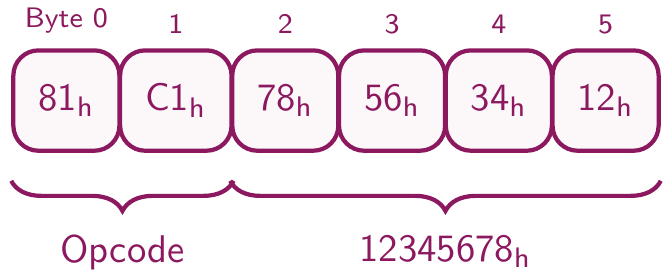
\includegraphics[width=0.1\textwidth]{opcode.png}

\section{Byte Order}
Stellen innerhalb Bytes werden nicht vertauscht!
\begin{description}
    \item[Big-Endian] CA | FE -> MSB ist erstes Bit
    \item[Little-Endian] FE | CA -> LSB ist erstes Bit
\end{description}

\section{Assembly}
\begin{description}
    \item[db] Byte, 8 Bit
    \item[dw] Word, 2 Byte, 16 Bit
    \item[dd] Doubleword, 4 Byte, 32 Bit
    \item[dq] Quadword, 8 Byte, 64 Bit
    \item [Double Quadword] 16 Byte, 128 Bit
\end{description}

\subsection{Labels}
\begin{lstlisting}[language={[x86masm]Assembler}]
text_length: dq after_my_text - my_text
my_text: db 'BSys 1'
after_my_text:
\end{lstlisting}

\subsection{Register}
\begin{tabular}{llllll}
    63..0 & 31..0 & 15..0 & 15..8 & 7..0\\
    \hline
    RAX & EAX & AX & AH & AL\\
\end{tabular}

\textbf{Weitere:} RCX, RDX, RBX, RSI, RDI, RSP, RBP, R8-R15

\subsection{Assembly Instructions}
\begin{description}
    \item mov rax, 1 \textcolor{teal}{//move the value 1 into rax}
    \item add z,   q  \textcolor{teal}{// z + q}
    \item sub z,   q  \textcolor{teal}{// z - q}
    \item adc z,   q  \textcolor{teal}{// z + q + c (carry -> previous calculation)}
    \item sbb z,   q  \textcolor{teal}{// z - q - c (carry -> previous calculation)}
    \item neg z       \textcolor{teal}{// 0 - z ("zweierkomplement")}
    \item inc z       \textcolor{teal}{// z++ }
    \item dec z       \textcolor{teal}{// z-- }
    \item mul rbx     \textcolor{teal}{// RBX * RAX. Ergebnis in RDX \& RAX }
    \item imul z      \textcolor{teal}{// signed equivalent for mul, z * RAX }
    \item div rbx      \textcolor{teal}{// RAX / RBX. Ergebnis: RAX. Rest: RDX. \underline{Slow}.}
    \item shl z,   i  \textcolor{teal}{// \(z * 2^i\) shift: <<}
    \item shr z,   i  \textcolor{teal}{// \(z * 2^{-i}\) z signed, shift: >>}
    \item sar z,   i  \textcolor{teal}{// \(z * 2^{-i}\) z unsigned, shift: >>, sign extension}
    \item rol z,   i  \textcolor{teal}{// Left-Rotate i Bits }
    \item ror z,   i  \textcolor{teal}{// Right-Rotate i Bits }
    \item and rax, rbx\textcolor{teal}{// AND}
    \item not rax     \textcolor{teal}{// NOT}
    \item test rax, rax \textcolor{teal}{// set ZF = 1 if rax == 0}
    \item cmp rax, 3 \textcolor{teal}{// compare rax and 3, set ZF = 1 if equal}
    \item cmove rax, 5 \textcolor{teal}{// move 5 into rax if equal}
    \item je 230 \textcolor{teal}{// move 230 down if condition met, RIP + 230, gemessen von Ende momentaner Instruktion}
    \item jmp S       \textcolor{teal}{// Jump to label S > GOTO}
    \item call S \textcolor{teal}{// push rax and jmp S > function call}
    \item ret    \textcolor{teal}{// pop rax and jmp rax > return}
\end{description}

\section{Flags}
CF \& OF werden immer beide von CPU bestimmt.

\begin{description}
    \item[Carry Flag (CF)] Überlauf bei \textbf{unsigned} Arithmetik
    0001 + 1111 = 0000, CF = 1 --> 1 + 15 = 0, CF = 1
    \item[Overflow Flag (OF)] Überlauf bei \textbf{signed} Arithmetik
    0111 + 0001 = 1000 -> 7 + 1 = -8 (negative prefix)
    \item[Zero Flag (ZF)] set when result is 0
    \item[Sign Flag] is the highest bit of the result (what is sign)
\end{description}

\subsection{Usage of compare with Condition Codes}
\textcolor{teal}{A : Above } \textcolor{teal}{ -> CF = 0 AND ZF = 0 \textbf{(unsigned)}}\newline
\textcolor{teal}{AE: Above or Equal } \textcolor{teal}{ -> CF = 0 \textbf{(unsigned)}}\newline
\textcolor{teal}{B : Below } \textcolor{teal}{ -> CF = 1 \textbf{(unsigned)}}\newline
\textcolor{teal}{BE: Below or Equal } \textcolor{teal}{ -> CF = 1 AND ZF = 1 \textbf{(unsigned)}}\newline
\textcolor{teal}{E : Equal } \textcolor{teal}{ -> ZF = 1}\newline
\textcolor{teal}{G : Greater } \textcolor{teal}{ -> SF = OF = 0 AND ZF = 0 \textbf{(signed)}}\newline
\textcolor{teal}{GE: Greater or Equal } \textcolor{teal}{ -> SF = OF \textbf{(signed)}}\newline
\textcolor{teal}{L : Less } \textcolor{teal}{ -> SF != OF \textbf{(signed)}}\newline
\textcolor{teal}{LE: Less or Equal } \textcolor{teal}{ -> SF != OF AND ZF = 1 \textbf{(signed)}}\newline
\textcolor{teal}{PE: Parity Even}  \textcolor{teal}{ -> PF = 1}\newline
\textcolor{teal}{PO: Parity Old } \textcolor{teal}{ -> PF = 0}\newline
\textcolor{teal}{Z:  Zero} \textcolor{teal}{ -> ZF = 1}

\section{Syscall}
\begin{lstlisting}[language={[x86masm]Assembler}]
mov rax, 60 ; 60 == exit instruction
mov rdi, 0 ; exit code -> 0 means ok
syscall ; OS executes instruction from rax
\end{lstlisting}

\section{Memory}
% TODO do I have enough space to add Displacement Adressierung, Scaled-Index-Adressierung & Base Adressierung?
\begin{lstlisting}[language={[x86masm]Assembler}]
mov rax, [0x8000] ; move 8000h into rax
mov rbx, [rax] ; address is in the register rax
mov [0x8000], rax ; move val at rax into 0x8000
mov rax, rbx ; rbx into rax, no memory access
mov [0x8000], [0x7000] ; err. can't move memory to memory
\end{lstlisting}
Operanden müssen gleich gross sein.

\section{Stack (\& Framepointer)}
Top Element at smallest address -> top to bottom

Prozessor überprüft \textbf{keine} obere/untere Grenze!

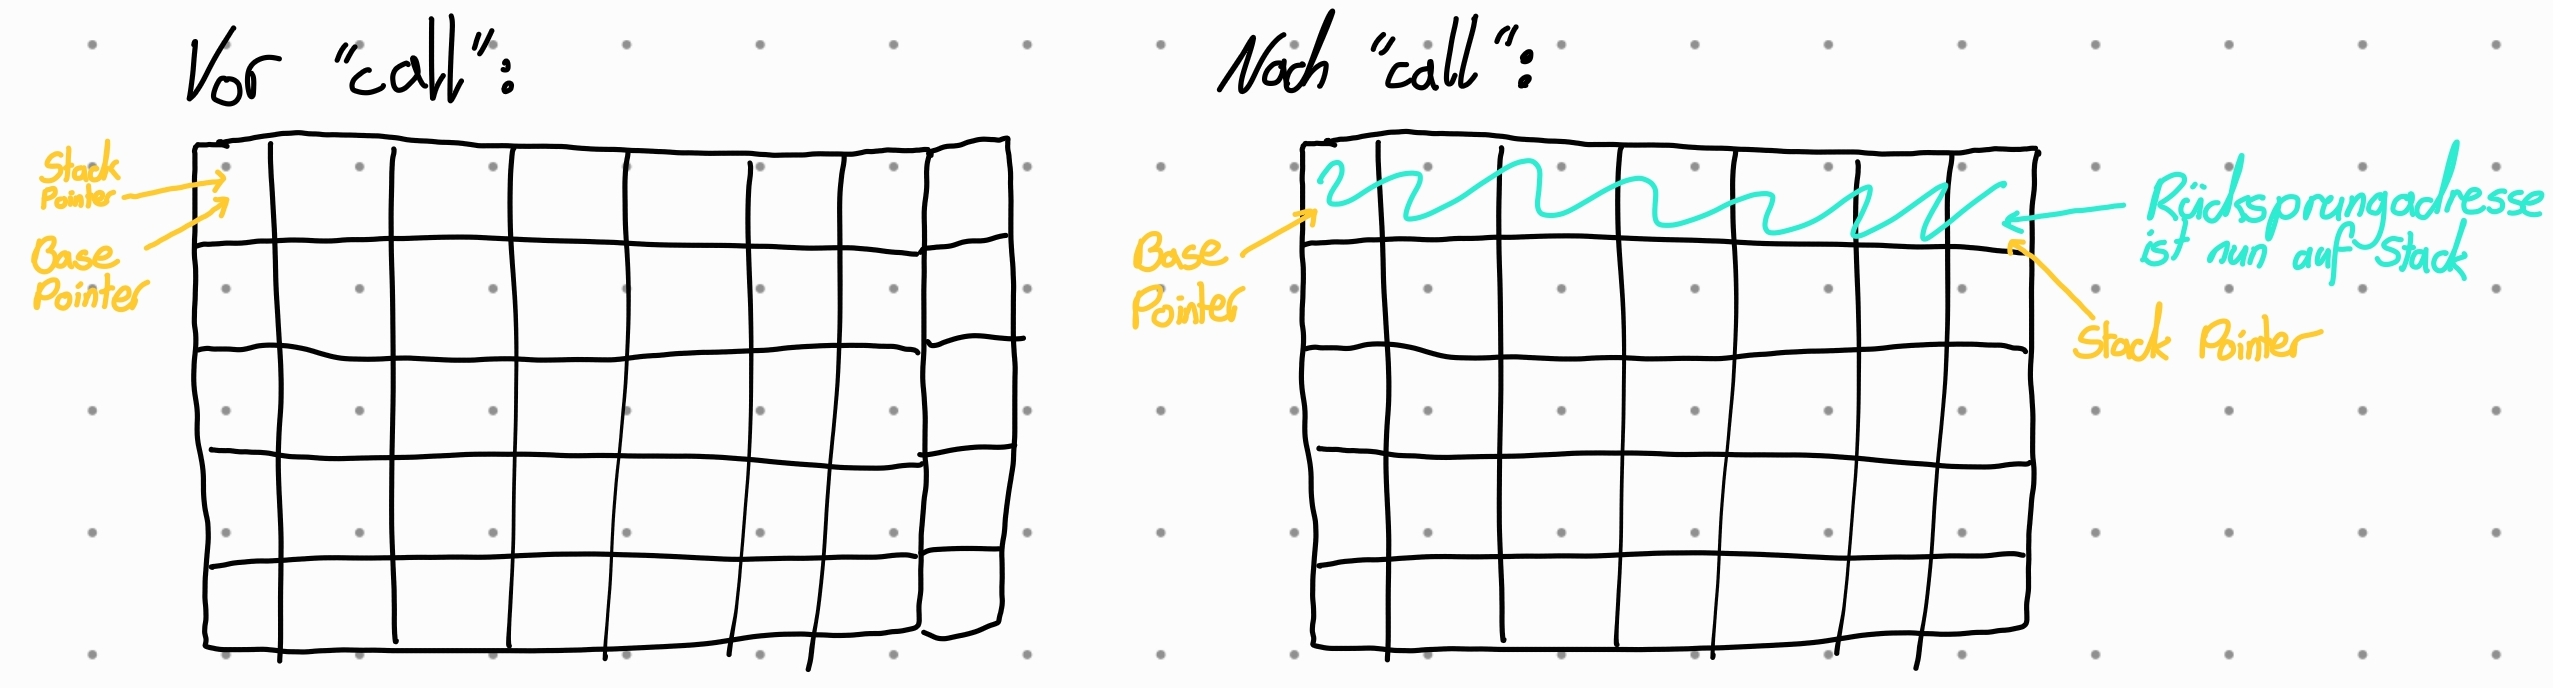
\includegraphics[width=0.25\textwidth]{rbp_rsp_base_sit.jpg}
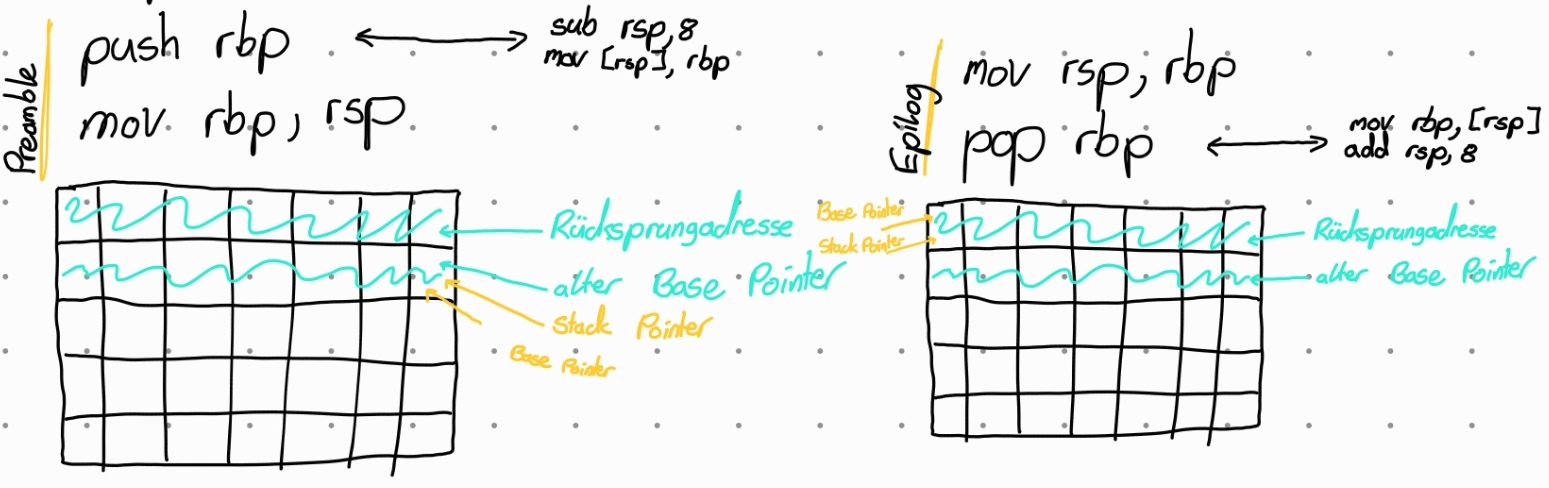
\includegraphics[width=0.25\textwidth]{rbp_rsp_preamble_epilogue.jpg}

Argumente sind vor der Rücksprungadresse auf Stack gelandet. Access via: [rbp + 0x10]

\section{Calling Conventions}
Welche Register / Stack für Argumente. Von Betriebssystem \& Compiler bestimmt => unterschiedlich

\section{C}
\subsection{C-Toolchain}
\begin{enumerate}
    \item \textbf{C Präprozessor} -> Bereinigte C-Quelle
    \item \textbf{C Compiler} -> Assembler Datei
    \item \textbf{Assembler} -> Objekt Datei
    \item \textbf{Linker} -> Executable
\end{enumerate}
\subsubsection{Präprozessor}
\begin{enumerate}
    \item Kommentare entfernen \& \ Zeilen zusammensetzen
    \item In Tokens aufteilen (Whitespace, bei a+b nicht nötig, String wird nicht aufgeteilt).

    Bildet grösstmögliches Token
    \item Präprozessor Direktiven ausführen (include, if, ...)
    \& Makros expandieren

    \cinline{#define XYZ 123 // XYZ wird im Folgenden mit 123 ersetzt}
\end{enumerate}


\subsubsection{Compiler}
Eine C-Datei -> Eine Assemblerdatei

Bezeichner dürfen beliebig oft \underline{deklariert} (int y;) werden. Nur 1x \underline{definiert} (int y = 5;).

\textbf{static}: Variable, die nicht exportiert werden soll

\begin{lstlisting}[language=c]
extern int x; static int x = 5; // Error:
// static Deklaration folgt auf non-static
\end{lstlisting}

Für globale Var wird Speicher fix reserviert. Grösse hängt von Typ ab. globale Var werden exportiert.

\subsubsection{Linker}
Mehrere Assemblerdateien -> Ein Executable

\subsection{Typen, sizeof(t)}
Typinfos nur auf C Sprachlevel

Size infos are dependent on architecture

\subsection{Vorzeichen}
Bei signed MSB: 0=positiv, 1=negativ

Umwandlung von negativer Binärzahl:

Zweierkomplement: flip + 1 (e.g. 1010 -> 0101 -> 0110)

\subsection{Pointers}

\begin{lstlisting}[language=c]
int a = 42;
int *b = &a; // b pointer to a
a = *b + 1; // a = dereference b and add 1
\end{lstlisting}
Incrementing a pointer will skip \textbf{sizeof(t)} Bytes!
\begin{lstlisting}[language=c]
int32_t x;
int32_t *y = &x;
y++; // y wird um 4 erhöht!
\end{lstlisting}
\vspace{2pt}
Pointer Differenz/Addition \textbf{nur} bei gleichen Typen!
\begin{lstlisting}[language=c]
int32_t *y = 100;
int32_t *x = 120;
prtdiff_t z = x - y; // z == 5 (5 * 4 Byte)
\end{lstlisting}

\subsection{Bitwise Operators}
Werden Bit per Bit angewendet:

not: \~{}q | and: q \& p | or: q | p

left shift: q << p (\(* 2^m\)) | right shift: q >> p ("\(/ 2^m\)")

\subsection{Logische Operatoren}
not: !q | and: q \&\& p | or: q || p

\subsection{Arithmetische Operationen}
z = x + y -> falls Überlauf: verpufft (kein Carry)

\subsection{Funktionen}
Parameter werden immer kopiert. (call by value)\vspace{2pt}

Bei Pointer als Parameter: Pointer wird kopiert, nicht der Wert dahinter -> Simulation von call by reference.\vspace{2pt}

Rückgabewert kann jeder Typ ausser Array Typen sein. Rückgabewert wird immer kopiert.

\begin{lstlisting}[language=c]
void f ();
void g (void);
f(); // OK
g(); // OK
f(1, 2, 3); // OK. LOL.
g(1, 2, 3); // Fehler -> parameter type is void
\end{lstlisting}

\subsection{printf Identifiers}
\begin{itemize}
    \item \textcolor{teal}{\textbf{sizeof(Integer)} as signed decimal = \%d oder \%i}
    \item \textcolor{teal}{\textbf{sizeof(Integer)} as unsigned decimal = \%u}
    \item \textcolor{teal}{\textbf{sizeof(Integer)} as hexadecimal = \%x or \%U}
    \item \textcolor{teal}{\textbf{sizeof(long)} as signed decimal = \%li}
    \item \textcolor{teal}{\textbf{sizeof(void *)} as pointer = \%p (hexadecimal)}
    \item \textcolor{teal}{\textbf{sizeof(char *)} as pointer (null terminated) = \%s}
    \item \textcolor{teal}{\textbf{sizeof(double)} as floating point = \%f}
\end{itemize}

\subsection{Datentypen}
Vordefinierte int Typen Aliase:

\cinline{intpr\_t}: Signed Integer Typ in den Adresse passt

\cinline{int8\_t}, \cinline{int16\_t}, \cinline{int32\_t}, \cinline{int64\_t}: Genaue Anzahl der Bits

\cinline{size\_t}: unsigned int -> genug gross für Adressierung von allem Speicher. Sicherer Datentyp iterieren Array.

\subsection{Arrays}
Label of Array used like \textbf{constant} Pointer

\cinline{int32_t a[10]} wird nicht initialisiert (ausser global)

\cinline{int a[4] = { 0x10 }} wird initialisiert

\cinline{a[0]=0x42} ist das gleiche wie \cinline{*a = 0x42}

\subsubsection{Arrays als Parameter}
\begin{itemize}
    \item Werden als Addressen übergeben, auch wenn Parameter als Array Typ deklariert wird
    \item Enthalten \textbf{keine} Information über ihre Grösse
\end{itemize}

\subsection{Strings}
\cinline{char * s = "Hai";} -> \textbf{Literal}, stored at special place, replaced with value of address, can't be changed, additional memory needed for pointer

\cinline{char c[] = \{'H', 'a', 'i', '\0'\};} -> size is compiled into program with sizeof (with function call, info is lost, as only pointer is given), values can be changed, 'c' is just a label that points to first index

Strings werden als char *s übergeben -> Null terminiert = wir wissen wo sie aufhören

\subsubsection{String Funktionen}
Länge von String: \cinline{strlen (char const *str)}, jedoch potenziell gefährlich wenn zB kein \textbackslash0 kommt

Deshalb: \cinline{strnlen (char const *str, size_t max)}: Bricht nach max Zeichen ab


\subsection{const}
von compiler überprüft, Tricks jedoch möglich, ausser global (Segmentation Fault)\vspace{2pt}

von rechts nach links lesen
\cinline{char const * const * c}\newline c is (non-const) pointer to const pointer to const char
\vspace{4pt}
wenn 'const' ganz links: \cinline{const char} <=> \cinline{char const}

\subsection{structs}
\begin{lstlisting}[language=c]
struct T // <- T ist der Tag.
{
    int x; // <- same address as struct
    int a[2]; // compiler can add padding
    char * name;
};
// If not enough members: Initialized with 0:
struct T t1 = { 2, {4, 5}, "Frida"};
struct T t2 = { .x = 2, .a[0] = 4, .a[1] = 5,
    .name = "Frida" }; // Explicit init
t1.x = 3;
struct T *t3 = &t2;
t3->x = 5; // only for pointers
\end{lstlisting}

\section{Cache}
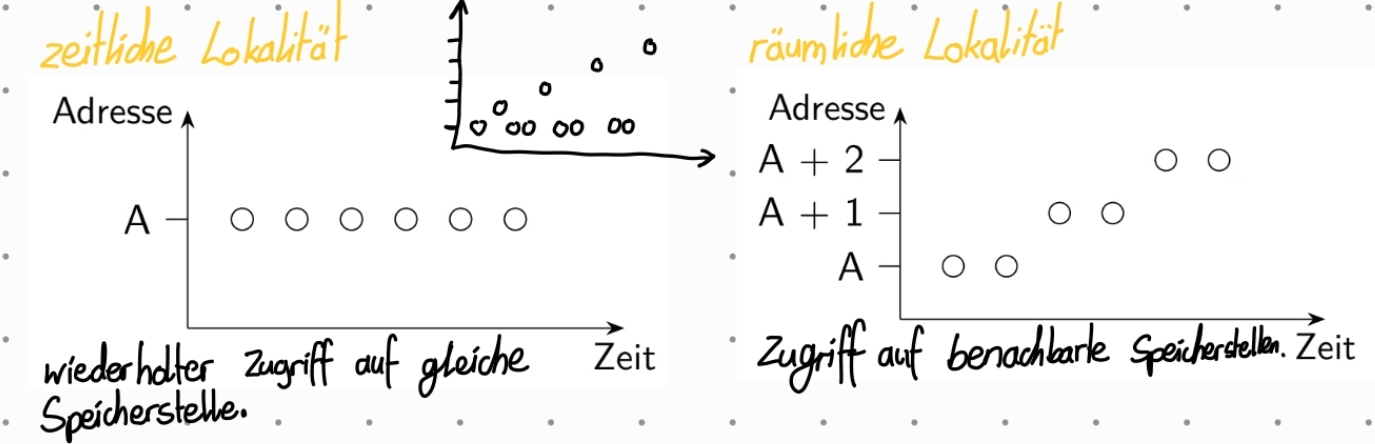
\includegraphics[width=0.24\textwidth]{locality.jpg}

\(E(T) = P_C * T_C + (1 - P_C )* T_M\)

\(T_C\): Access time on Cache |
\(T_M\): Access time on Memory |
\(P_C\): Probability of Cache-Hit

\subsection{Fully Associative Cache (FAC)}
Every Cache Row mapped to 1 address on cache.

e.g. for 64 Byte: n-6 upper Bits for identifying cache line. \& lower 6 bits for \textbf{offset} in a cache line

e.g.: \((84480801_h / 2^4) / 2^2 = 8448080_h / 2^2 = 2112020_h\)

\textbf{One} lookup hardware part \textbf{per entry}! Parts compare at same time if match exists. High costs, really fast.

\subsection{Direct Mapped Cache (DMC)}

Adresse hat fixen Platz in Liste: untere p Bits identifizieren Zeile/Index. Unterste für \textbf{Offset} in Cache Line

Nur reduzierter Tag wird gespeichert (Tag ohne untere p Bits). Braucht nur einen Baustein für Vergleich.

einfach zu implementieren, schneller Lookup, viele Kollisionen (\(1234_h\), \(AB34_h\), p=8 -> beide in Eintrag \(34_h\))

\begin{description}
    \item[Offset Bits] = Zeilengrösse (16 B -> \(2^4\) -> 4 Bit)
    \item[Bits für Zeilen] = Total Daten / Cachezeilenlänge
    \item[Tag Bits] = Adressbits - Bits für Zeilen - Offset Bits
\end{description}

\subsection{k-Way Set-Associative Cache}
Mehrere (k) Direct Mapped Caches -> weniger Kollisionen als DMC, weniger komplex als FAC

Grösse von Way = Total / Anzahl Ways

\section{Dynamischer Speicher}
Heap: Speicherbereich für vollständig dynamischen Speicher. Reservierter Speicher \textbf{muss} freigegeben werden (explizit/implizit).

\begin{lstlisting}[language=c]
void * malloc (size_t s)
void free (void * p)
\end{lstlisting}

easy variant for knowing how much memory to free:
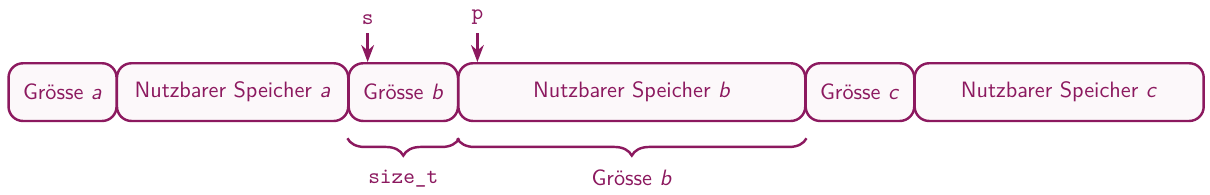
\includegraphics[width=0.24\textwidth]{implementation_memory.png}

\subsection{Fragmentierung}
\textbf{Interne Fragmentierung}: Heap reserviert mehr Speicher als angeforder (zB immer Vielfache von 8)

\textbf{Externe Fragmentierung}: immer wieder Speicher reserviert, unregelmässig freigeben

-> nur noch kleine Löcher

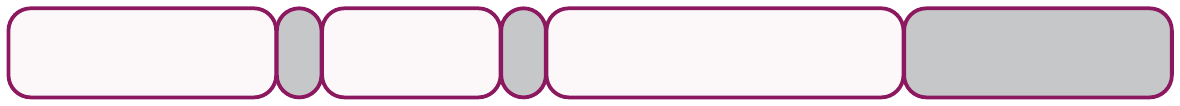
\includegraphics[width=0.2\textwidth]{external_fragmentation.png}

\subsection{Buddy System}

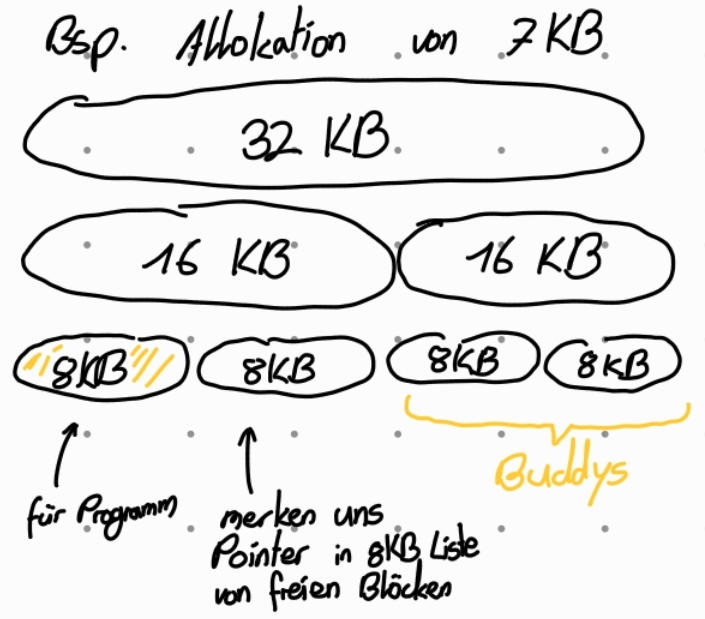
\includegraphics[width=0.12\textwidth]{buddies_1.jpg}

Wird Bereich freigegeben: Überprüfen ob Buddy in \(2^k\)-Liste mit Freielementen

\textbf{Nein}: Bereich hinzufügen zu Freielementen

\textbf{Ja}: Buddy aus Freiliste entfernen, Bereich mergen, mit Freigabe (rekursiv) fortfahren

Buddies wenn: gleiche Grösse, Startadresse darf sich nur im Bit k unterscheiden!

% Idea is to add some small notes with pencil on the left
\hfill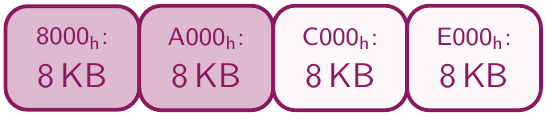
\includegraphics[width=0.12\textwidth]{buddies_2.png}

\subsection{Suchalgorithmen für freie Bereiche}
\begin{description}
    \item[First Fit] Erste passende Lücke am Anfang
    \item[Next Fit] Erste passende Lücke \underline{nach} zuletzt reserviertem Bereich
    \item[Best Fit] Durchsucht \underline{alle} Lücken, wählt kleinste aus
    \item[Worst Fit] Durchsucht \underline{alle} Lücken, wählt grösste aus
    \item[Quick Fit] Erstes, kleinstes Element aus Liste
    (Rekombination ist schwierig)
\end{description}

\subsection{in Linux}
Buddy-System für grosse Blöcke. Kleinste Blockgrösse = 4KB. malloc für Benutzer Applikationen

\subsection{Objekt Pools}
Speicherbereich fester Grösse, wird in kleine Bereiche mit gleicher Grösse unterteilt.

\section{Memory Management Unit (MMU)}
Prozess erhält virtuelle und nicht reale Adresse von OS. MMU macht Übersetzung.

=> mehr Speicher von Prozess verwendbar als RAM vorhanden, keine Rücksicht auf andere Prozesse

\subsection{Fault Interrupt}
Fehlendes Mapping => MMU wirft Fault Interrupt => CPU ruft OS-Interrupt Handler auf \& OS übernimmt.\vspace{2pt}

Wenn RAM ausgelagert, Interrupt wird getriggered. OS lädt RAM nach, passt Mapping Table an, setzt Prozess fort.

\begin{description}
    \item[Page] typischerweise 4KB. Repräsentiert Daten. Kein Speicher, braucht Page Frame. OS platziert Pages.
    \item[Page Frame] Gleich gross wie Page (4KB)
    \item[Page Table] Virtuelle Adresse wird via Page-Table in reale Adresse übersetzt
\end{description}
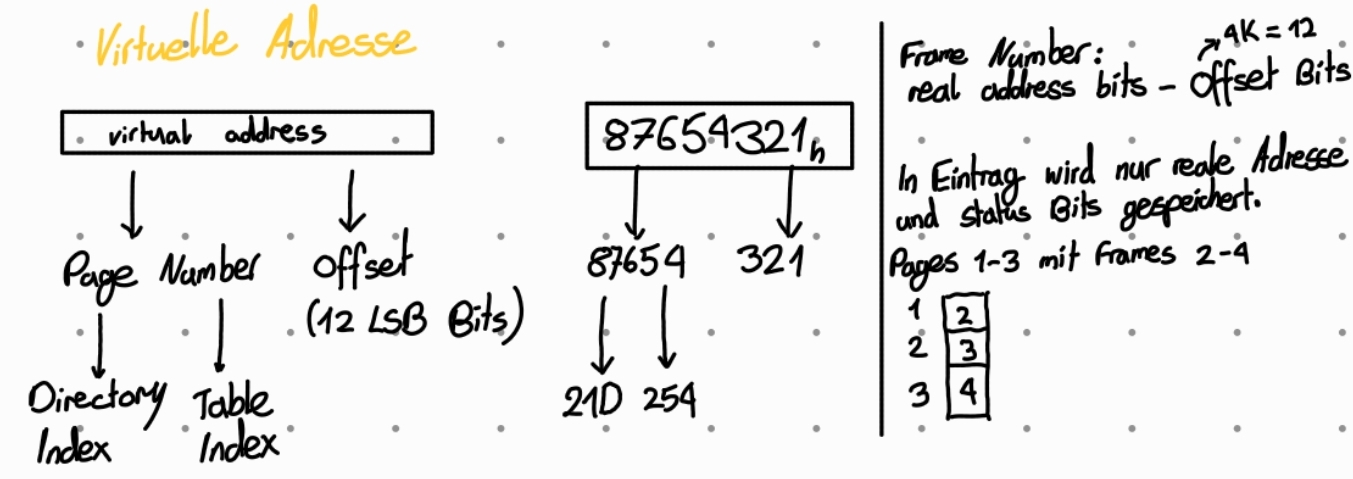
\includegraphics[width=0.21\textwidth]{virtual_address_to_index.jpg}

\subsection{Single-Level Page Table}
Index = Page Number. Grösse hängt von Grösse des virtuellen Adressraums ab.

Für jeden Prozess braucht es \underline{volle} Page Table. Auch wenn nur wenig Speicher benötigt.

\subsection{Multi-Level Page Tables}
Bei einer Table/Directory wird immer Speicher für ganze Liste gebraucht.

Tables die nicht gebraucht werden, werden nicht angelegt.

Status Bit "Used" in Table \& Directory gibt an ob genutzt. Wenn in Table alles auf 0: löschen.

\section{Virtueller Speicher (Software)}
\begin{description}
    \item[P-Bit] =1: Page ist im Speicher, =0: Page ist nicht im Speicher
    \item[A-Bit] =Accessed. Page wurde \underline{kürzlich} im Prozess verwendet. MMU setzt bei jedem Lesezugriff auf 1. OS soll es in Zeitintervallen löschen.
    \item[D-Bit] =Dirty. Page in RAM anders als in sekundären Speicher. OS soll erst löschen, wenn Page tatsächlich zurückgeschrieben wurde.
\end{description}
% TODO maybe add combinations? dependent on space.
\vspace{2pt}
Wenn nicht im Hauptspeicher:
\begin{enumerate}
    \item MMU wirft Fault Interrupt
    \item OS schaut "Page Location Information" an. gültig -> lade page. ungültig -> segmentation fault
\end{enumerate}

Problem: Häufiges Paging (Threshing). Verminderung durch Paging-Strategien / mehr Ram / max. Anzahl Prozesse

\subsection{Ladestrategien}
\begin{description}
    \item[Demand Paging] Pages nur dann geladen, wenn benötigt. Braucht immer Interrupt
    \item[Prepaging] Seiten werden vor Verwendung geladen. (in Reinform muss Zukunft bekannt sein)
    \item[Demand Paging mit Prepaging] Benachbarte Pages in Clustern mitgeladen (zB 4 oder 8)
    -> weniger Page Faults, Blocktransfer, vlt nicht benötigte Pages geladen
\end{description}

\subsection{Entladestrategien (wann zurück in Swap?)}
\begin{description}
    \item[Demand Cleaning] Page wird zurückgeschrieben, wenn Frame ersetzt werden soll
    \item[Precleaning] Modifizierte Pages werden frühzeitig in sekundären Speicher geschrieben.
    Bei Page Wechsel muss alte Page nicht mehr geschrieben werden. Wenn Page nochmals verändert: Schreiben vergebens.
\end{description}

\subsection{Verdrängungsstrategien}
Wenn Speicher knapp: welche Page aus Hauptspeicher entfernt? Sauber/D=0 Pages bevorzugt ersetzen

\begin{description}
    \item[Optimal] Page die am spätesten wieder benötigt wird
    \item[FIFO] First in First Out
    \item[Second Chance] Älteste nicht verwendete Page wird entfernt. Wenn alle Pages verwendet=FIFO. Neue Page hat A=1. In Kreis verhängte LinkedList.
    \item[Least Recently Used] am längsten unbenutzte Page. MMU muss Zeitpunkt in Page-Table notieren. Page mit kleinstem T wird ersetzt. Hoher HW Aufwand.
    \item[Not Frequently Used] OS misst A-Bits in regelmässigem Abstand. Counter Table. In Timer-Interrupt wird Counter erhöht, falls Zugriff passiert. Problem: Alte Pages können lange drin bleiben.  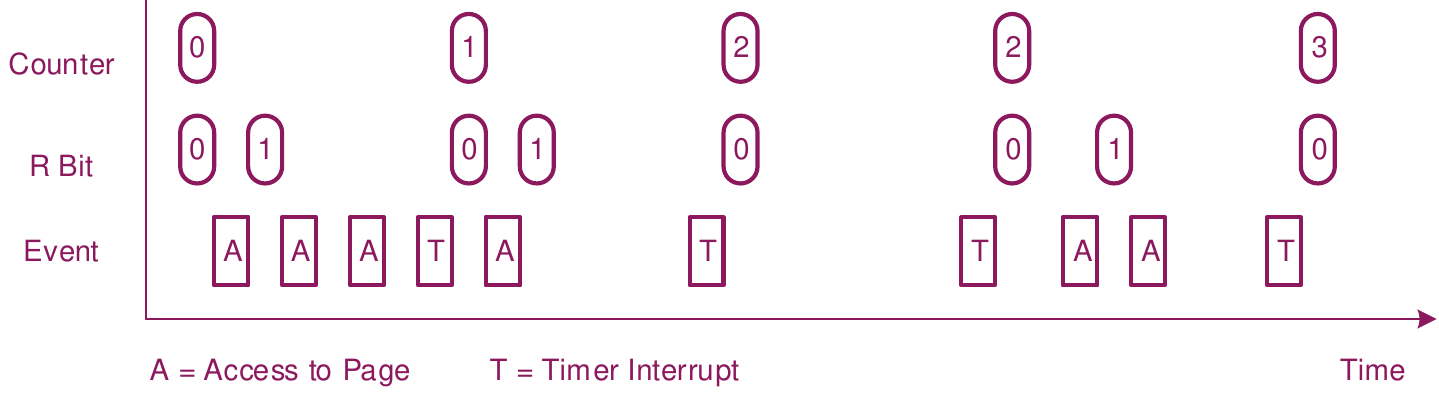
\includegraphics[width=0.21\textwidth]{nfu.png}
    \item[NFU mit Aging] Counter wird mit Bit Shifting gealtert 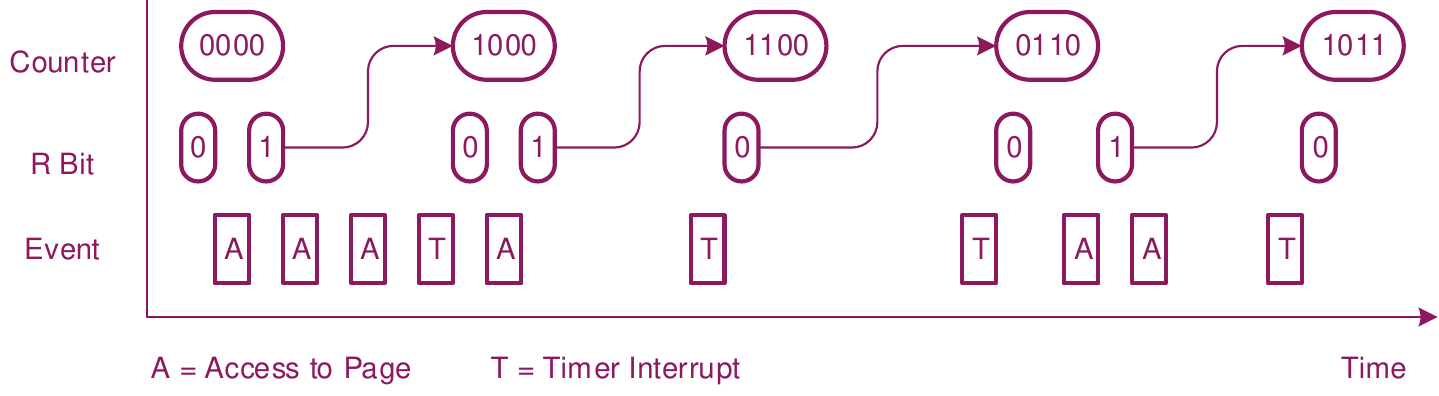
\includegraphics[width=0.2\textwidth]{nfu_aging.png}
    \item[Working Set] Scanne \underline{alle} Pages in Fault Interrupt. Behalte Pages von aktuellem Working Set, Limit für Alter ist Intervall T, Zeitstempel in Page Table eingetragen. Wenn keine Page gefunden: älteste Page (D=0 bevorzugt)
    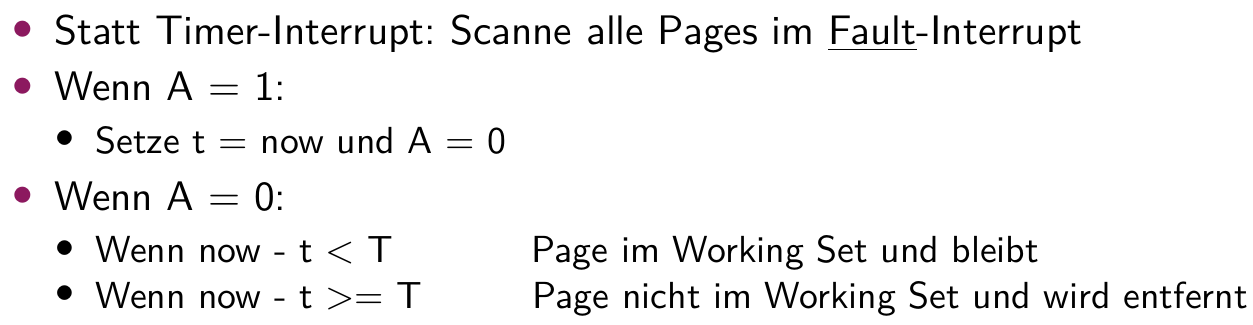
\includegraphics[width=0.21\textwidth]{working_set.png}
    \item[WSClock] Wie Working Set \underline{ABER} in Kreis verhängte LinkedList: In Kreis herumgehen, nächste Page zum Entfernen suchen.
\end{description}


\end{multicols*}
\end{document}